In this section, we document the details of the event yield and BDT 
distributions after the Higgs selections in the multivariate based analysis. 
Figure~\ref{fig:mva_115_4700pb}-\ref{fig:mva_140_4700pb} show the BDT 
output distributions comparing data with the signal and background predictions, for 
the $mH=115-140$ \GeVcc.


\begin{table}[!ht]
{%\footnotesize
 \tiny
 \begin{center}
 \begin{tabular}{l c c c c c c c c c c c }
 \hline
 mH & ggH & qqWW & ggWW & VV & Top & Zjets & Wjets & Wgamma & Ztt & $\sum$Bkg & Data \\
 \hline
110 & $3.0\pm0.7$ & $99.8\pm10.1$ & $4.5\pm1.4$ & $2.2\pm0.2$ & $6.3\pm1.3$ & $0.6\pm0.1$ & $21.2\pm7.6$ & $6.6\pm2.0$ & $0.1\pm0.0$ & $141.3\pm13.0$ & 140 \\
115 & $7.4\pm1.6$ & $122.5\pm12.4$ & $5.7\pm1.8$ & $2.6\pm0.2$ & $8.2\pm1.7$ & $0.6\pm0.1$ & $23.8\pm8.6$ & $7.4\pm2.3$ & $0.1\pm0.0$ & $171.0\pm15.5$ & 176 \\
120 & $14.4\pm3.2$ & $144.4\pm14.6$ & $7.1\pm2.2$ & $3.0\pm0.2$ & $9.6\pm2.0$ & $0.6\pm0.1$ & $26.4\pm9.5$ & $7.8\pm2.4$ & $0.1\pm0.0$ & $198.9\pm17.9$ & 202 \\
130 & $40.6\pm8.8$ & $209.5\pm21.6$ & $10.5\pm3.3$ & $4.1\pm0.3$ & $15.5\pm3.2$ & $0.7\pm0.1$ & $33.1\pm11.9$ & $9.2\pm2.8$ & $0.2\pm0.0$ & $282.9\pm25.3$ & 285 \\
140 & $78.4\pm16.9$ & $279.6\pm29.1$ & $15.4\pm4.9$ & $5.3\pm0.4$ & $23.0\pm4.8$ & $0.8\pm0.1$ & $38.7\pm13.9$ & $10.3\pm3.2$ & $0.2\pm0.0$ & $373.4\pm33.1$ & 360 \\
150 & $117.8\pm25.9$ & $332.7\pm36.4$ & $19.4\pm6.2$ & $6.4\pm0.5$ & $31.5\pm6.6$ & $0.9\pm0.1$ & $41.7\pm15.0$ & $11.4\pm3.5$ & $0.2\pm0.0$ & $444.1\pm40.6$ & 436 \\
160 & $167.8\pm36.8$ & $354.4\pm38.8$ & $22.1\pm7.1$ & $6.7\pm0.5$ & $35.2\pm7.4$ & $0.9\pm0.1$ & $43.8\pm15.8$ & $11.4\pm3.5$ & $0.2\pm0.0$ & $474.8\pm43.3$ & 465 \\
170 & $168.1\pm37.6$ & $367.9\pm40.3$ & $24.2\pm7.7$ & $7.0\pm0.5$ & $38.4\pm8.1$ & $1.0\pm0.1$ & $44.9\pm16.1$ & $11.5\pm3.5$ & $0.2\pm0.0$ & $494.9\pm45.0$ & 493 \\
180 & $141.4\pm31.6$ & $381.3\pm43.9$ & $25.5\pm8.2$ & $7.7\pm0.6$ & $45.4\pm9.5$ & $1.0\pm0.1$ & $47.6\pm17.1$ & $12.6\pm3.8$ & $0.2\pm0.0$ & $521.2\pm48.9$ & 540 \\
190 & $104.5\pm23.8$ & $411.9\pm49.0$ & $27.3\pm8.8$ & $8.2\pm0.6$ & $51.5\pm10.8$ & $1.0\pm0.1$ & $51.5\pm18.5$ & $13.6\pm4.2$ & $0.2\pm0.0$ & $565.4\pm54.4$ & 581 \\
200 & $79.2\pm18.0$ & $396.0\pm71.3$ & $25.8\pm8.9$ & $8.7\pm0.6$ & $56.8\pm11.9$ & $1.1\pm0.1$ & $53.4\pm19.2$ & $14.0\pm4.3$ & $0.3\pm0.0$ & $556.0\pm75.4$ & 610 \\
250 & $45.4\pm11.1$ & $490.4\pm88.2$ & $30.1\pm10.4$ & $10.8\pm0.8$ & $83.9\pm17.6$ & $1.2\pm0.1$ & $62.5\pm22.5$ & $15.0\pm4.6$ & $0.3\pm0.0$ & $694.2\pm93.4$ & 760 \\
300 & $30.7\pm8.1$ & $501.1\pm90.1$ & $30.7\pm10.6$ & $11.0\pm0.8$ & $88.0\pm18.5$ & $1.2\pm0.1$ & $63.8\pm23.0$ & $15.0\pm4.6$ & $0.3\pm0.0$ & $711.2\pm95.6$ & 774 \\
350 & $27.7\pm8.2$ & $506.6\pm91.1$ & $30.9\pm10.7$ & $11.2\pm0.8$ & $89.5\pm18.8$ & $1.2\pm0.1$ & $64.5\pm23.2$ & $15.0\pm4.6$ & $0.3\pm0.0$ & $719.2\pm96.6$ & 780 \\
400 & $21.1\pm6.1$ & $509.1\pm91.6$ & $31.1\pm10.8$ & $11.2\pm0.8$ & $90.3\pm19.0$ & $1.2\pm0.1$ & $64.5\pm23.2$ & $15.2\pm4.7$ & $0.3\pm0.0$ & $722.8\pm97.1$ & 783 \\
450 & $12.9\pm4.2$ & $510.2\pm91.8$ & $31.1\pm10.8$ & $11.3\pm0.8$ & $90.7\pm19.0$ & $1.2\pm0.1$ & $64.4\pm23.2$ & $15.6\pm4.8$ & $0.3\pm0.0$ & $724.7\pm97.3$ & 783 \\
500 & $7.8\pm2.9$ & $510.9\pm91.9$ & $31.2\pm10.8$ & $11.3\pm0.8$ & $90.7\pm19.1$ & $1.2\pm0.1$ & $64.4\pm23.2$ & $15.6\pm4.8$ & $0.3\pm0.0$ & $725.6\pm97.4$ & 787 \\
550 & $5.0\pm2.1$ & $511.3\pm92.0$ & $31.2\pm10.8$ & $11.3\pm0.8$ & $90.8\pm19.1$ & $1.2\pm0.1$ & $64.7\pm23.3$ & $15.6\pm4.8$ & $0.3\pm0.0$ & $726.4\pm97.5$ & 787 \\
600 & $3.1\pm1.5$ & $511.7\pm92.1$ & $31.2\pm10.8$ & $11.3\pm0.8$ & $91.0\pm19.1$ & $1.2\pm0.1$ & $64.7\pm23.3$ & $15.6\pm4.8$ & $0.3\pm0.0$ & $726.8\pm97.6$ & 787 \\
\hline
\end{tabular}
\end{center}
}
\caption{Summary of the yields after the mva selections in the 0-Jet bin opposite flavor ($e\mu$) final states corresponding to \intlumi\ data. The uncertainties include 
both statistical and systematic contributions. }
%\end{table}
%\begin{table}[!ht]
{%\footnotesize
 \tiny
 \begin{center}
 \begin{tabular}{l c c c c c c c c c c c }
 \hline
 mH & ggH & qqWW & ggWW & VV & Top & Zjets & Wjets & Wgamma & Ztt & $\sum$Bkg & Data \\
 \hline
110 & $0.9\pm0.2$ & $62.5\pm6.3$ & $2.5\pm0.8$ & $1.1\pm0.1$ & $3.5\pm0.7$ & $9.7\pm5.3$ & $5.3\pm1.9$ & $0.9\pm0.3$ & $0.0\pm0.0$ & $85.5\pm8.6$ & 81 \\
115 & $2.8\pm0.6$ & $81.8\pm8.3$ & $3.4\pm1.1$ & $1.4\pm0.1$ & $4.9\pm1.0$ & $11.2\pm6.1$ & $6.8\pm2.4$ & $0.9\pm0.3$ & $0.0\pm0.0$ & $110.4\pm10.7$ & 108 \\
120 & $6.3\pm1.4$ & $101.5\pm10.3$ & $4.4\pm1.4$ & $1.7\pm0.1$ & $6.2\pm1.3$ & $11.7\pm6.1$ & $7.7\pm2.8$ & $0.9\pm0.3$ & $0.0\pm0.0$ & $134.0\pm12.4$ & 128 \\
130 & $22.6\pm4.9$ & $145.5\pm15.0$ & $6.9\pm2.2$ & $2.5\pm0.2$ & $9.8\pm2.1$ & $13.0\pm6.2$ & $11.6\pm4.2$ & $0.9\pm0.3$ & $0.0\pm0.0$ & $190.1\pm17.0$ & 199 \\
140 & $48.1\pm10.4$ & $177.7\pm18.5$ & $9.0\pm2.9$ & $2.8\pm0.2$ & $12.9\pm2.7$ & $15.0\pm6.9$ & $13.6\pm4.9$ & $0.9\pm0.3$ & $0.0\pm0.0$ & $232.0\pm20.7$ & 237 \\
150 & $80.5\pm17.7$ & $194.6\pm21.3$ & $10.9\pm3.5$ & $3.2\pm0.2$ & $16.1\pm3.4$ & $18.0\pm8.4$ & $14.1\pm5.1$ & $0.9\pm0.3$ & $0.0\pm0.0$ & $257.8\pm24.0$ & 264 \\
160 & $125.5\pm27.6$ & $208.9\pm22.9$ & $12.6\pm4.0$ & $3.4\pm0.2$ & $18.8\pm3.9$ & $18.6\pm8.4$ & $15.1\pm5.4$ & $0.9\pm0.3$ & $0.0\pm0.0$ & $278.2\pm25.6$ & 278 \\
170 & $125.9\pm28.1$ & $217.8\pm23.9$ & $13.7\pm4.4$ & $3.5\pm0.3$ & $20.7\pm4.4$ & $19.3\pm8.5$ & $14.9\pm5.4$ & $1.1\pm0.3$ & $0.0\pm0.0$ & $291.1\pm26.6$ & 290 \\
180 & $104.3\pm23.3$ & $217.7\pm25.1$ & $14.1\pm4.5$ & $3.7\pm0.3$ & $22.9\pm4.8$ & $20.5\pm8.7$ & $15.7\pm5.7$ & $1.6\pm0.5$ & $0.0\pm0.0$ & $296.2\pm27.9$ & 313 \\
190 & $68.5\pm15.6$ & $239.1\pm28.4$ & $15.5\pm5.0$ & $4.0\pm0.3$ & $26.6\pm5.6$ & $21.8\pm8.8$ & $16.3\pm5.9$ & $2.0\pm0.6$ & $0.0\pm0.0$ & $325.3\pm31.3$ & 345 \\
200 & $50.7\pm11.5$ & $232.8\pm41.9$ & $14.8\pm5.1$ & $4.3\pm0.3$ & $29.5\pm6.2$ & $22.6\pm8.8$ & $17.1\pm6.2$ & $2.3\pm0.7$ & $0.0\pm0.0$ & $323.5\pm44.0$ & 375 \\
250 & $24.4\pm6.0$ & $303.0\pm54.5$ & $17.9\pm6.2$ & $5.5\pm0.4$ & $47.4\pm10.0$ & $26.6\pm9.5$ & $19.9\pm7.2$ & $3.4\pm1.0$ & $0.0\pm0.0$ & $423.8\pm57.0$ & 507 \\
300 & $18.0\pm4.8$ & $309.7\pm55.7$ & $18.4\pm6.4$ & $5.7\pm0.4$ & $49.6\pm10.4$ & $27.6\pm9.6$ & $20.5\pm7.4$ & $3.9\pm1.2$ & $0.0\pm0.0$ & $435.4\pm58.3$ & 518 \\
350 & $17.6\pm5.2$ & $312.9\pm56.3$ & $18.7\pm6.5$ & $5.8\pm0.4$ & $50.6\pm10.6$ & $28.2\pm9.6$ & $21.1\pm7.6$ & $5.4\pm1.7$ & $0.0\pm0.0$ & $442.5\pm58.9$ & 521 \\
400 & $13.4\pm3.9$ & $314.3\pm56.5$ & $18.7\pm6.5$ & $5.8\pm0.4$ & $51.1\pm10.7$ & $28.6\pm9.6$ & $21.4\pm7.7$ & $5.4\pm1.7$ & $0.0\pm0.0$ & $445.4\pm59.2$ & 521 \\
450 & $8.3\pm2.7$ & $315.0\pm56.7$ & $18.7\pm6.5$ & $5.8\pm0.4$ & $51.3\pm10.8$ & $28.8\pm9.6$ & $21.4\pm7.7$ & $5.4\pm1.7$ & $0.0\pm0.0$ & $446.4\pm59.4$ & 524 \\
500 & $5.1\pm1.9$ & $315.3\pm56.7$ & $18.7\pm6.5$ & $5.9\pm0.4$ & $51.3\pm10.8$ & $28.9\pm9.6$ & $21.4\pm7.7$ & $5.4\pm1.7$ & $0.0\pm0.0$ & $447.0\pm59.4$ & 525 \\
550 & $3.2\pm1.4$ & $315.5\pm56.8$ & $18.8\pm6.5$ & $5.9\pm0.4$ & $51.4\pm10.8$ & $29.0\pm9.6$ & $21.5\pm7.7$ & $5.4\pm1.7$ & $0.0\pm0.0$ & $447.4\pm59.5$ & 526 \\
600 & $2.0\pm1.0$ & $315.7\pm56.8$ & $18.8\pm6.5$ & $5.9\pm0.4$ & $51.4\pm10.8$ & $29.0\pm9.6$ & $21.5\pm7.7$ & $5.4\pm1.7$ & $0.0\pm0.0$ & $447.6\pm59.5$ & 526 \\
\hline
\end{tabular}
\end{center}
}
\caption{Summary of the yields after the mva selections in the 0-Jet bin same flavor (ee and $\mu\mu$) final states corresponding to \intlumi\ data. The uncertainties include 
both statistical and systematic contributions. }
\end{table}
\begin{table}[!ht]
{%\footnotesize
 \tiny
 \begin{center}
 \begin{tabular}{l c c c c c c c c c c c }
 \hline
 mH & ggH & qqWW & ggWW & VV & Top & Zjets & Wjets & Wgamma & Ztt & $\sum$Bkg & Data \\
 \hline
110 & $1.3\pm0.4$ & $31.4\pm4.5$ & $1.5\pm0.5$ & $2.9\pm0.2$ & $19.0\pm1.2$ & $0.6\pm0.1$ & $13.1\pm4.7$ & $1.5\pm0.5$ & $0.4\pm0.0$ & $70.3\pm6.6$ & 80 \\
115 & $3.0\pm1.0$ & $37.8\pm5.4$ & $1.8\pm0.6$ & $3.2\pm0.2$ & $23.3\pm1.4$ & $0.6\pm0.1$ & $15.0\pm5.4$ & $1.7\pm0.5$ & $0.4\pm0.0$ & $83.8\pm7.8$ & 91 \\
120 & $5.5\pm1.8$ & $44.6\pm6.3$ & $2.2\pm0.7$ & $3.5\pm0.3$ & $27.5\pm1.7$ & $0.6\pm0.1$ & $15.6\pm5.6$ & $1.7\pm0.5$ & $0.4\pm0.0$ & $96.2\pm8.7$ & 103 \\
130 & $15.9\pm5.3$ & $64.8\pm9.6$ & $3.5\pm1.2$ & $4.8\pm0.3$ & $43.1\pm2.6$ & $1.0\pm0.1$ & $20.7\pm7.4$ & $1.7\pm0.5$ & $0.5\pm0.1$ & $140.2\pm12.5$ & 145 \\
140 & $31.8\pm10.2$ & $93.8\pm13.4$ & $5.6\pm1.8$ & $6.1\pm0.4$ & $62.0\pm3.8$ & $1.2\pm0.1$ & $25.0\pm9.0$ & $1.9\pm0.6$ & $0.6\pm0.1$ & $196.0\pm16.7$ & 189 \\
150 & $44.9\pm14.2$ & $118.3\pm17.8$ & $7.2\pm2.4$ & $7.0\pm0.5$ & $82.4\pm5.0$ & $1.2\pm0.1$ & $27.7\pm10.0$ & $2.1\pm0.6$ & $0.7\pm0.1$ & $246.7\pm21.2$ & 227 \\
160 & $69.4\pm21.9$ & $130.7\pm19.7$ & $8.1\pm2.7$ & $7.3\pm0.5$ & $93.1\pm5.7$ & $1.3\pm0.1$ & $27.8\pm10.0$ & $2.1\pm0.6$ & $0.8\pm0.1$ & $271.1\pm23.0$ & 244 \\
170 & $72.7\pm22.8$ & $139.0\pm20.8$ & $8.9\pm3.0$ & $7.5\pm0.5$ & $101.8\pm6.2$ & $1.3\pm0.1$ & $27.8\pm10.0$ & $2.1\pm0.6$ & $0.8\pm0.1$ & $289.1\pm24.1$ & 259 \\
180 & $65.2\pm20.3$ & $146.4\pm23.4$ & $9.4\pm3.2$ & $8.3\pm0.6$ & $117.4\pm7.2$ & $1.4\pm0.1$ & $29.1\pm10.5$ & $2.1\pm0.6$ & $0.8\pm0.1$ & $314.8\pm26.9$ & 293 \\
190 & $50.0\pm15.6$ & $163.4\pm26.8$ & $10.2\pm3.5$ & $9.0\pm0.6$ & $130.5\pm8.0$ & $1.4\pm0.1$ & $31.7\pm11.4$ & $2.1\pm0.6$ & $0.8\pm0.1$ & $349.0\pm30.4$ & 323 \\
200 & $37.5\pm11.3$ & $145.5\pm30.6$ & $8.9\pm3.1$ & $9.5\pm0.7$ & $140.7\pm8.6$ & $1.5\pm0.1$ & $33.1\pm11.9$ & $2.1\pm0.6$ & $0.8\pm0.1$ & $342.1\pm34.1$ & 342 \\
250 & $24.0\pm7.2$ & $188.1\pm39.6$ & $10.8\pm3.8$ & $12.1\pm0.9$ & $190.3\pm11.6$ & $1.6\pm0.2$ & $40.8\pm14.7$ & $3.0\pm0.9$ & $0.9\pm0.1$ & $447.8\pm44.0$ & 446 \\
300 & $17.8\pm5.4$ & $195.1\pm41.0$ & $11.2\pm3.9$ & $12.5\pm0.9$ & $197.0\pm12.0$ & $2.1\pm0.2$ & $42.3\pm15.2$ & $3.0\pm0.9$ & $0.9\pm0.1$ & $464.2\pm45.6$ & 461 \\
350 & $17.9\pm5.6$ & $198.0\pm41.7$ & $11.4\pm3.9$ & $12.7\pm0.9$ & $200.6\pm12.2$ & $2.1\pm0.2$ & $42.6\pm15.3$ & $3.0\pm0.9$ & $0.9\pm0.1$ & $471.3\pm46.2$ & 469 \\
400 & $14.5\pm4.5$ & $200.5\pm42.2$ & $11.5\pm4.0$ & $12.8\pm0.9$ & $201.8\pm12.3$ & $2.1\pm0.2$ & $43.3\pm15.6$ & $3.0\pm0.9$ & $0.9\pm0.1$ & $475.9\pm46.8$ & 470 \\
450 & $9.3\pm3.1$ & $201.7\pm42.4$ & $11.6\pm4.0$ & $12.8\pm0.9$ & $202.5\pm12.4$ & $2.1\pm0.2$ & $43.5\pm15.6$ & $3.0\pm0.9$ & $0.9\pm0.1$ & $478.1\pm47.1$ & 473 \\
500 & $6.3\pm2.2$ & $202.4\pm42.6$ & $11.6\pm4.0$ & $12.9\pm0.9$ & $202.6\pm12.4$ & $2.1\pm0.2$ & $43.6\pm15.7$ & $3.0\pm0.9$ & $0.9\pm0.1$ & $479.2\pm47.2$ & 473 \\
550 & $4.0\pm1.6$ & $202.7\pm42.6$ & $11.6\pm4.0$ & $12.9\pm0.9$ & $202.8\pm12.4$ & $2.1\pm0.2$ & $43.6\pm15.7$ & $3.0\pm0.9$ & $0.9\pm0.1$ & $479.7\pm47.3$ & 474 \\
600 & $2.6\pm1.2$ & $202.8\pm42.7$ & $11.6\pm4.0$ & $12.9\pm0.9$ & $203.0\pm12.4$ & $2.1\pm0.2$ & $43.8\pm15.8$ & $3.0\pm0.9$ & $0.9\pm0.1$ & $480.2\pm47.3$ & 474 \\
\hline
\end{tabular}
\end{center}
}
\caption{Summary of the yields after the mva selections in the 1-Jet bin opposite flavor ($e\mu$) final states corresponding to \intlumi\ data. The uncertainties include 
both statistical and systematic contributions. }
%\end{table}
%\begin{table}[!ht]
{%\footnotesize
 \tiny
 \begin{center}
 \begin{tabular}{l c c c c c c c c c c c }
 \hline
 mH & ggH & qqWW & ggWW & VV & Top & Zjets & Wjets & Wgamma & Ztt & $\sum$Bkg & Data \\
 \hline
110 & $0.3\pm0.1$ & $13.8\pm2.0$ & $0.7\pm0.2$ & $0.8\pm0.1$ & $8.2\pm0.5$ & $17.0\pm3.2$ & $3.5\pm1.3$ & $0.3\pm0.1$ & $0.0\pm0.0$ & $44.4\pm4.0$ & 36 \\
115 & $0.9\pm0.3$ & $18.0\pm2.5$ & $0.9\pm0.3$ & $1.1\pm0.1$ & $10.9\pm0.7$ & $18.9\pm3.6$ & $4.4\pm1.6$ & $0.3\pm0.1$ & $0.0\pm0.0$ & $54.4\pm4.7$ & 47 \\
120 & $1.9\pm0.6$ & $21.9\pm3.1$ & $1.3\pm0.4$ & $1.3\pm0.1$ & $14.4\pm0.9$ & $21.0\pm4.0$ & $4.9\pm1.8$ & $1.1\pm0.3$ & $0.0\pm0.0$ & $66.0\pm5.4$ & 58 \\
130 & $6.8\pm2.2$ & $32.9\pm4.9$ & $2.0\pm0.7$ & $1.8\pm0.1$ & $23.3\pm1.4$ & $28.0\pm5.2$ & $5.6\pm2.0$ & $1.9\pm0.6$ & $0.0\pm0.0$ & $95.6\pm7.6$ & 97 \\
140 & $15.6\pm5.0$ & $45.5\pm6.5$ & $3.2\pm1.1$ & $2.0\pm0.1$ & $30.4\pm1.9$ & $28.3\pm5.2$ & $7.6\pm2.7$ & $2.0\pm0.6$ & $0.0\pm0.0$ & $119.0\pm9.0$ & 115 \\
150 & $26.8\pm8.5$ & $53.7\pm8.1$ & $3.9\pm1.3$ & $2.2\pm0.2$ & $38.1\pm2.3$ & $29.2\pm5.3$ & $7.8\pm2.8$ & $2.9\pm0.9$ & $0.0\pm0.0$ & $137.8\pm10.4$ & 134 \\
160 & $46.6\pm14.7$ & $60.5\pm9.1$ & $4.6\pm1.5$ & $2.4\pm0.2$ & $45.0\pm2.7$ & $31.1\pm5.7$ & $8.2\pm3.0$ & $2.9\pm0.9$ & $0.0\pm0.0$ & $154.8\pm11.6$ & 147 \\
170 & $47.8\pm15.0$ & $65.4\pm9.8$ & $5.0\pm1.7$ & $2.5\pm0.2$ & $50.5\pm3.1$ & $31.4\pm5.7$ & $8.4\pm3.0$ & $2.9\pm0.9$ & $0.0\pm0.0$ & $166.2\pm12.2$ & 159 \\
180 & $42.3\pm13.2$ & $66.8\pm10.7$ & $5.0\pm1.7$ & $2.7\pm0.2$ & $56.3\pm3.4$ & $34.3\pm6.1$ & $9.2\pm3.3$ & $3.1\pm1.0$ & $0.0\pm0.0$ & $177.4\pm13.4$ & 175 \\
190 & $26.8\pm8.4$ & $77.2\pm12.7$ & $5.6\pm1.9$ & $3.0\pm0.2$ & $64.5\pm3.9$ & $37.9\pm6.7$ & $9.7\pm3.5$ & $3.9\pm1.2$ & $0.0\pm0.0$ & $201.9\pm15.4$ & 193 \\
200 & $21.1\pm6.3$ & $69.7\pm14.7$ & $4.9\pm1.7$ & $3.3\pm0.2$ & $71.1\pm4.3$ & $39.2\pm6.9$ & $10.8\pm3.9$ & $4.1\pm1.2$ & $0.0\pm0.0$ & $203.1\pm17.3$ & 214 \\
250 & $11.3\pm3.4$ & $96.5\pm20.3$ & $6.2\pm2.1$ & $4.5\pm0.3$ & $100.8\pm6.1$ & $42.3\pm7.3$ & $12.7\pm4.6$ & $6.2\pm1.9$ & $0.0\pm0.0$ & $269.3\pm23.1$ & 290 \\
300 & $9.4\pm2.9$ & $100.2\pm21.1$ & $6.4\pm2.2$ & $4.7\pm0.3$ & $104.6\pm6.4$ & $42.8\pm7.3$ & $13.0\pm4.7$ & $6.3\pm1.9$ & $0.0\pm0.0$ & $277.9\pm23.8$ & 307 \\
350 & $9.4\pm2.9$ & $101.9\pm21.4$ & $6.5\pm2.2$ & $4.7\pm0.3$ & $105.9\pm6.5$ & $43.0\pm7.3$ & $13.4\pm4.8$ & $6.6\pm2.0$ & $0.0\pm0.0$ & $282.1\pm24.2$ & 312 \\
400 & $8.3\pm2.6$ & $102.9\pm21.6$ & $6.5\pm2.2$ & $4.8\pm0.3$ & $106.6\pm6.5$ & $43.2\pm7.3$ & $13.7\pm4.9$ & $6.6\pm2.0$ & $0.0\pm0.0$ & $284.3\pm24.5$ & 315 \\
450 & $5.5\pm1.8$ & $103.3\pm21.7$ & $6.5\pm2.3$ & $4.8\pm0.3$ & $107.0\pm6.5$ & $43.3\pm7.3$ & $13.8\pm5.0$ & $6.6\pm2.0$ & $0.0\pm0.0$ & $285.3\pm24.5$ & 316 \\
500 & $3.7\pm1.3$ & $103.7\pm21.8$ & $6.5\pm2.3$ & $4.8\pm0.3$ & $107.1\pm6.5$ & $43.3\pm7.3$ & $13.8\pm5.0$ & $6.6\pm2.0$ & $0.0\pm0.0$ & $286.1\pm24.6$ & 316 \\
550 & $2.4\pm1.0$ & $104.0\pm21.9$ & $6.5\pm2.3$ & $4.8\pm0.3$ & $107.2\pm6.5$ & $43.4\pm7.3$ & $13.9\pm5.0$ & $6.6\pm2.0$ & $0.0\pm0.0$ & $286.5\pm24.7$ & 317 \\
600 & $1.6\pm0.7$ & $104.1\pm21.9$ & $6.6\pm2.3$ & $4.8\pm0.3$ & $107.3\pm6.5$ & $43.4\pm7.3$ & $14.0\pm5.0$ & $6.6\pm2.0$ & $0.0\pm0.0$ & $286.8\pm24.7$ & 318 \\
\hline
\end{tabular}
\end{center}
}
\caption{Summary of the yields after the mva selections in the 1-Jet bin same flavor (ee and $\mu\mu$) final states corresponding to \intlumi\ data. The uncertainties include 
both statistical and systematic contributions. }
\end{table}

\clearpage

\begin{figure}[!hbtp]
\centering
\subfigure[]{
\centering
\label{subfig:mva_115_0j_of_4700pb}
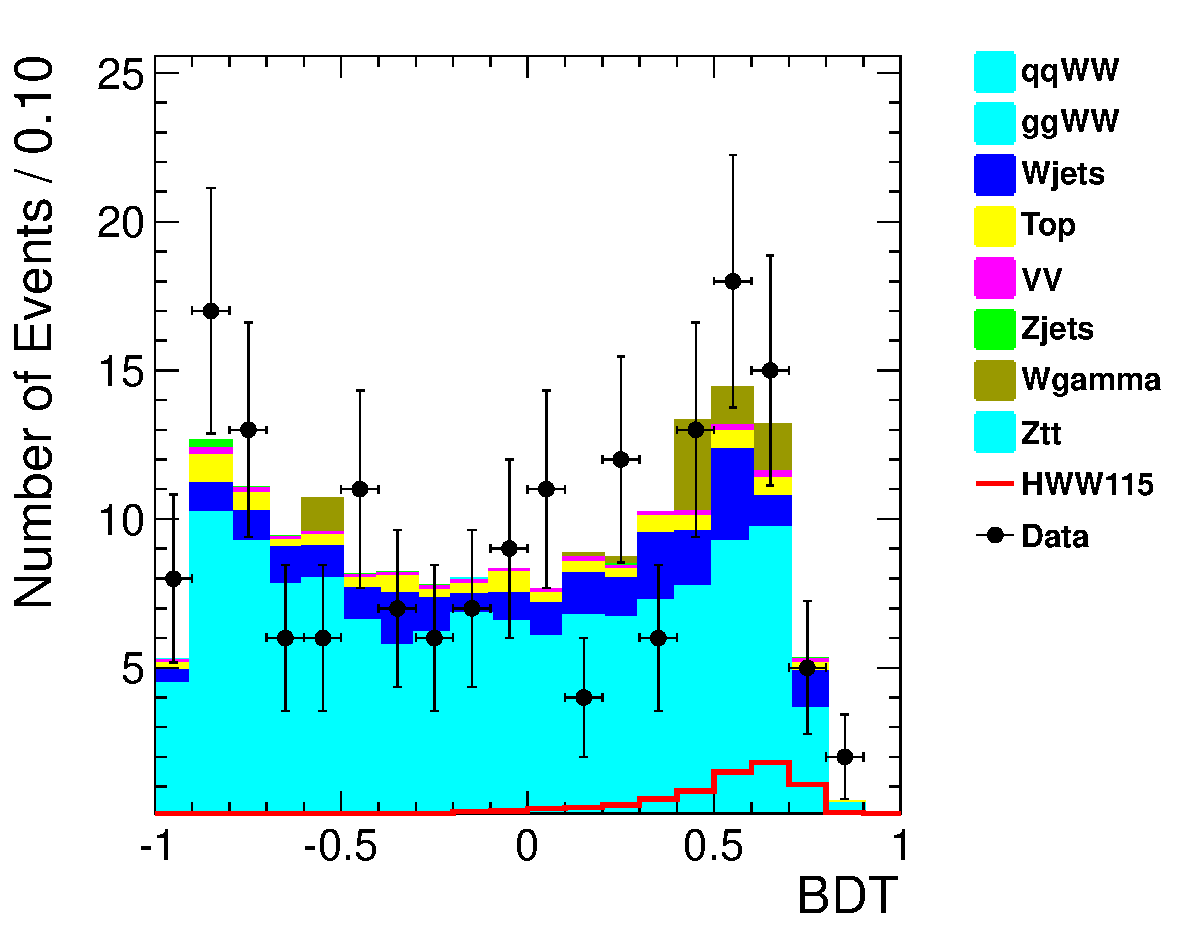
\includegraphics[width=.40\textwidth]{figures/BDT_mH115_0j_of_stack_lin.pdf}}
\subfigure[]{
\centering
\label{subfig:mva_115_0j_sf_4700pb}
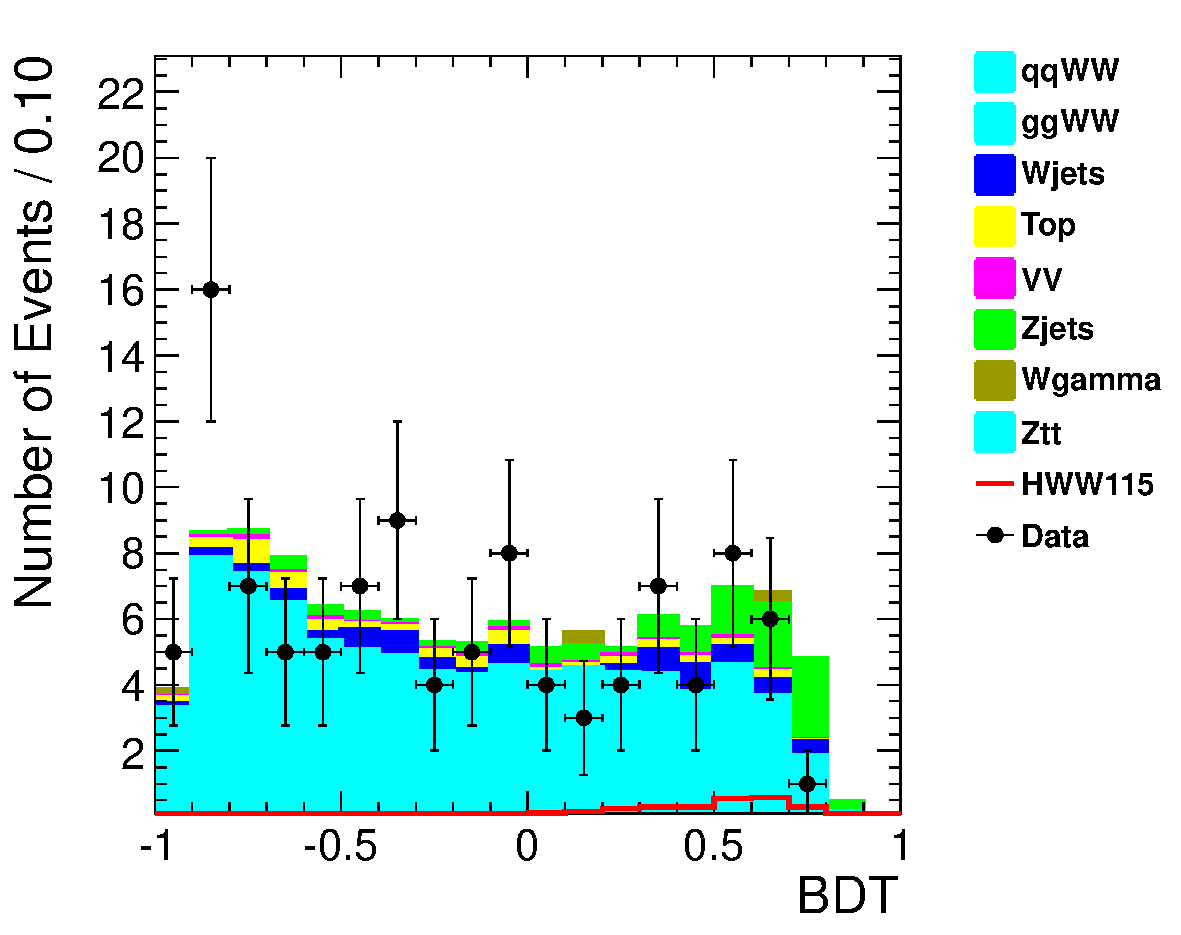
\includegraphics[width=.40\textwidth]{figures/BDT_mH115_0j_sf_stack_lin.pdf}}
\subfigure[]{
\centering
\label{subfig:mva_115_1j_of_4700pb}
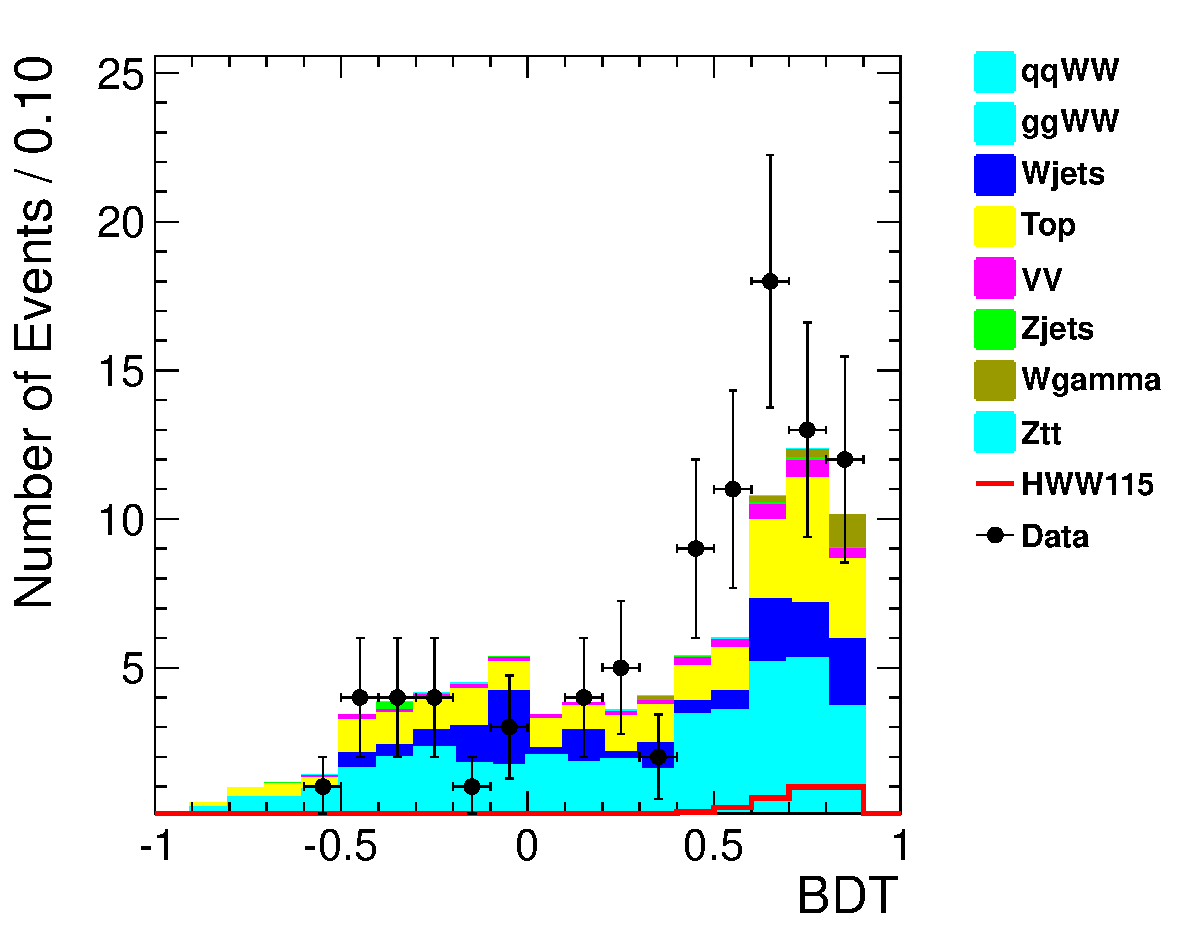
\includegraphics[width=.40\textwidth]{figures/BDT_mH115_1j_of_stack_lin.pdf}}
\subfigure[]{
\centering
\label{subfig:mva_115_1j_sf_4700pb}
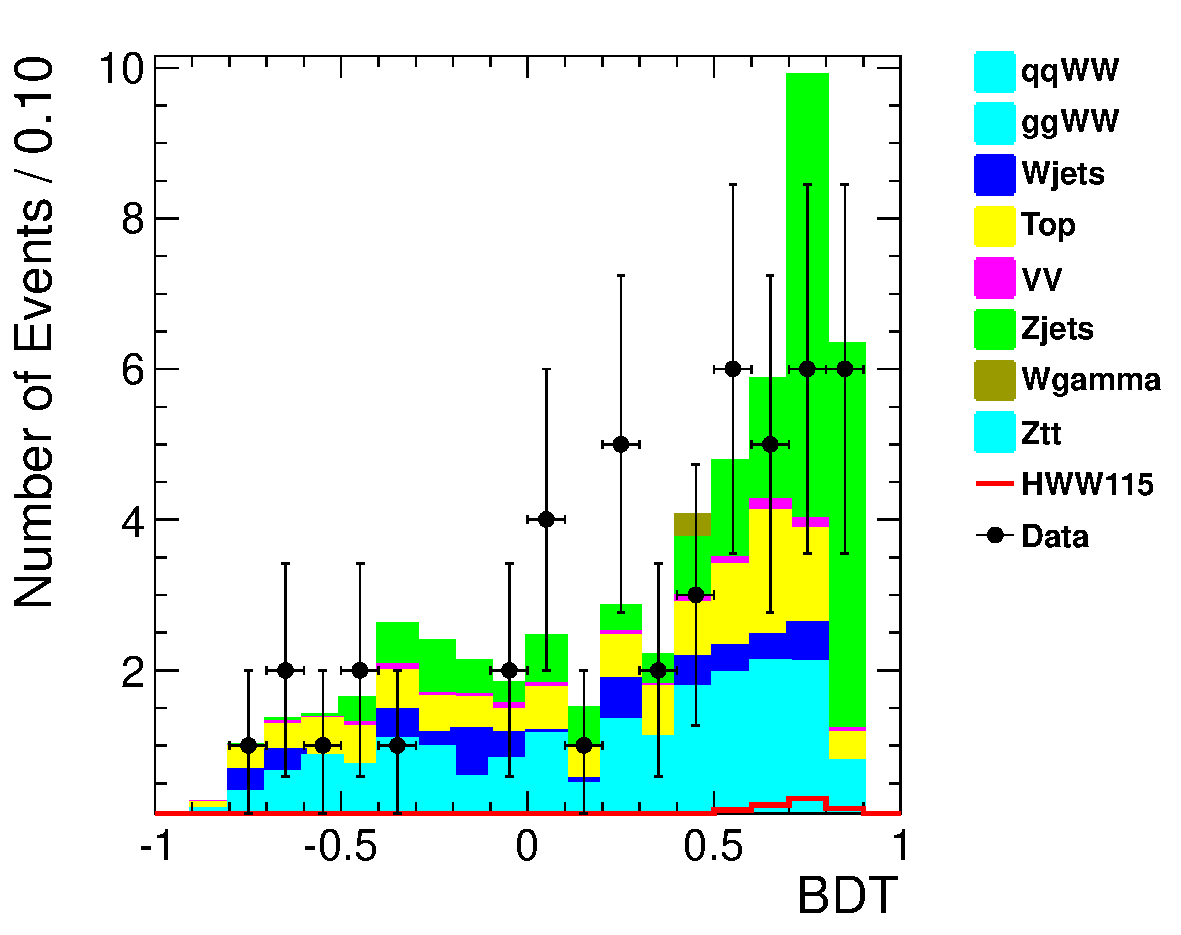
\includegraphics[width=.40\textwidth]{figures/BDT_mH115_1j_sf_stack_lin.pdf}}
\caption{
MVA output for $m_H$=115 GeV corresponding to \intlumi:
0-jet OF \subref{subfig:mva_115_0j_of_4700pb},
0-jet SF \subref{subfig:mva_115_0j_sf_4700pb},
1-jet OF \subref{subfig:mva_115_1j_of_4700pb},
1-jet SF \subref{subfig:mva_115_1j_sf_4700pb}
.}
\label{fig:mva_115_4700pb}
\end{figure}

\begin{figure}[!hbtp]
\centering
\subfigure[]{
\centering
\label{subfig:mva_120_0j_of_4700pb}
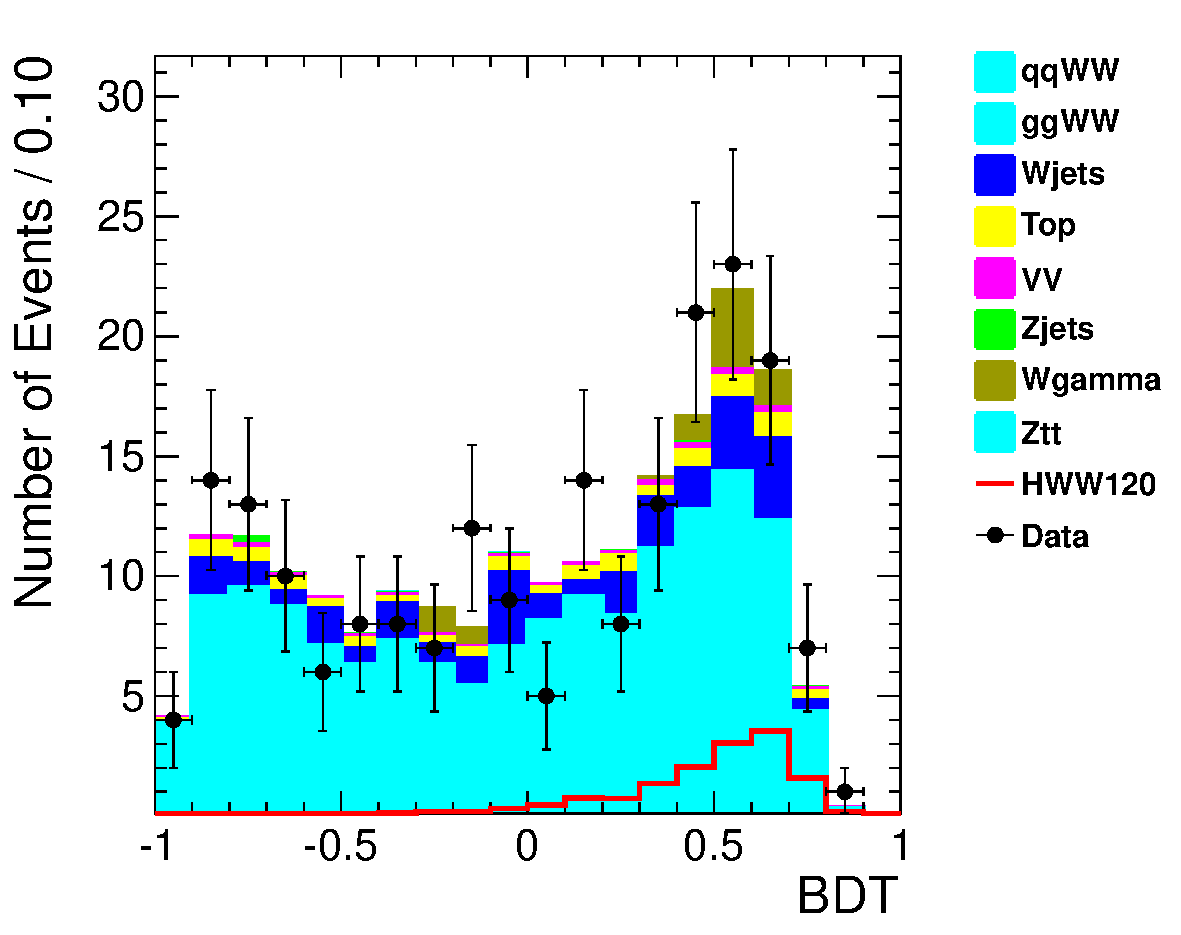
\includegraphics[width=.40\textwidth]{figures/BDT_mH120_0j_of_stack_lin.pdf}}
\subfigure[]{
\centering
\label{subfig:mva_120_0j_sf_4700pb}
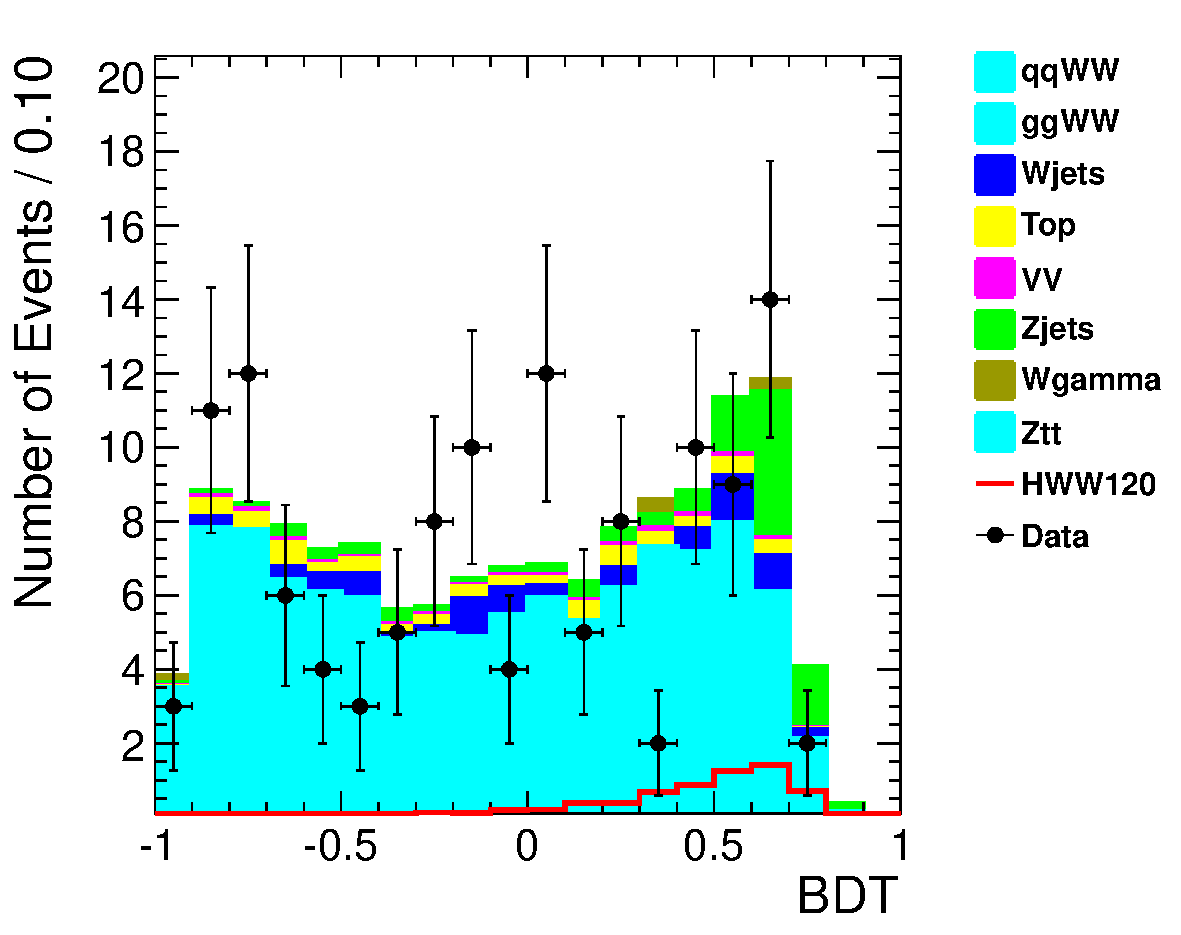
\includegraphics[width=.40\textwidth]{figures/BDT_mH120_0j_sf_stack_lin.pdf}}
\subfigure[]{
\centering
\label{subfig:mva_120_1j_of_4700pb}
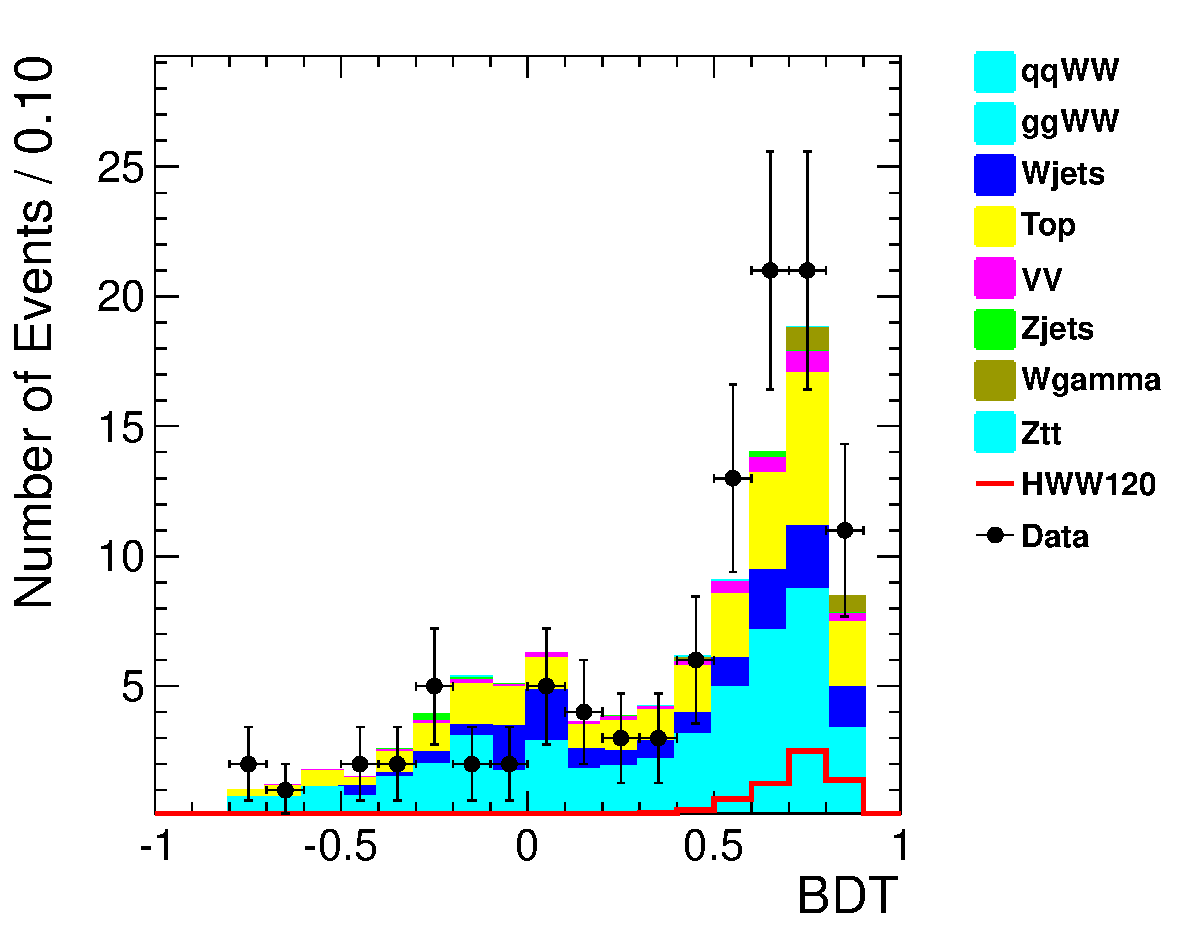
\includegraphics[width=.40\textwidth]{figures/BDT_mH120_1j_of_stack_lin.pdf}}
\subfigure[]{
\centering
\label{subfig:mva_120_1j_sf_4700pb}
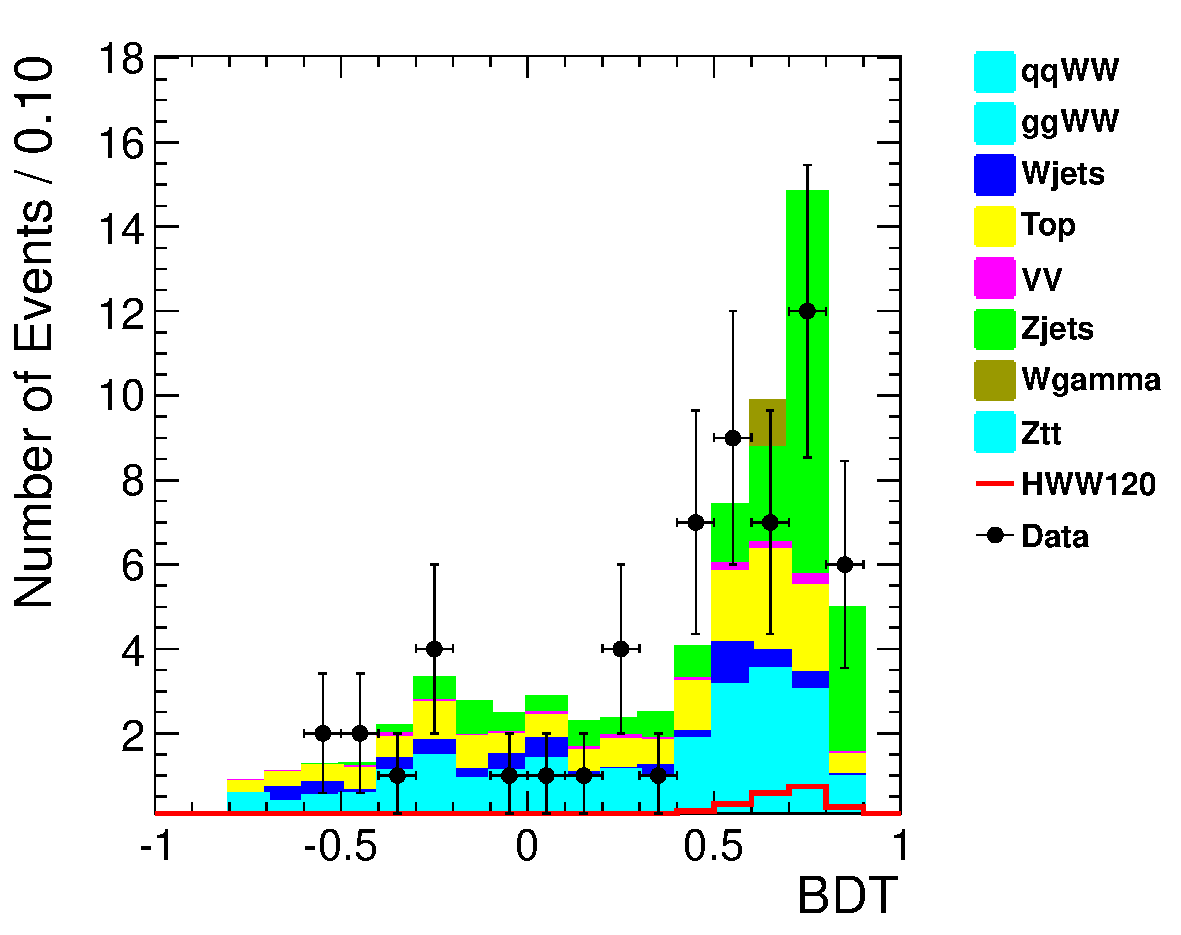
\includegraphics[width=.40\textwidth]{figures/BDT_mH120_1j_sf_stack_lin.pdf}}
\caption{
MVA output for $m_H$=120 GeV corresponding to \intlumi:
0-jet OF \subref{subfig:mva_120_0j_of_4700pb},
0-jet SF \subref{subfig:mva_120_0j_sf_4700pb},
1-jet OF \subref{subfig:mva_120_1j_of_4700pb},
1-jet SF \subref{subfig:mva_120_1j_sf_4700pb}
.}
\label{fig:mva_120_4700pb}
\end{figure}


\begin{figure}[!hbtp]
\centering
\subfigure[]{
\centering
\label{subfig:mva_130_0j_of_4700pb}
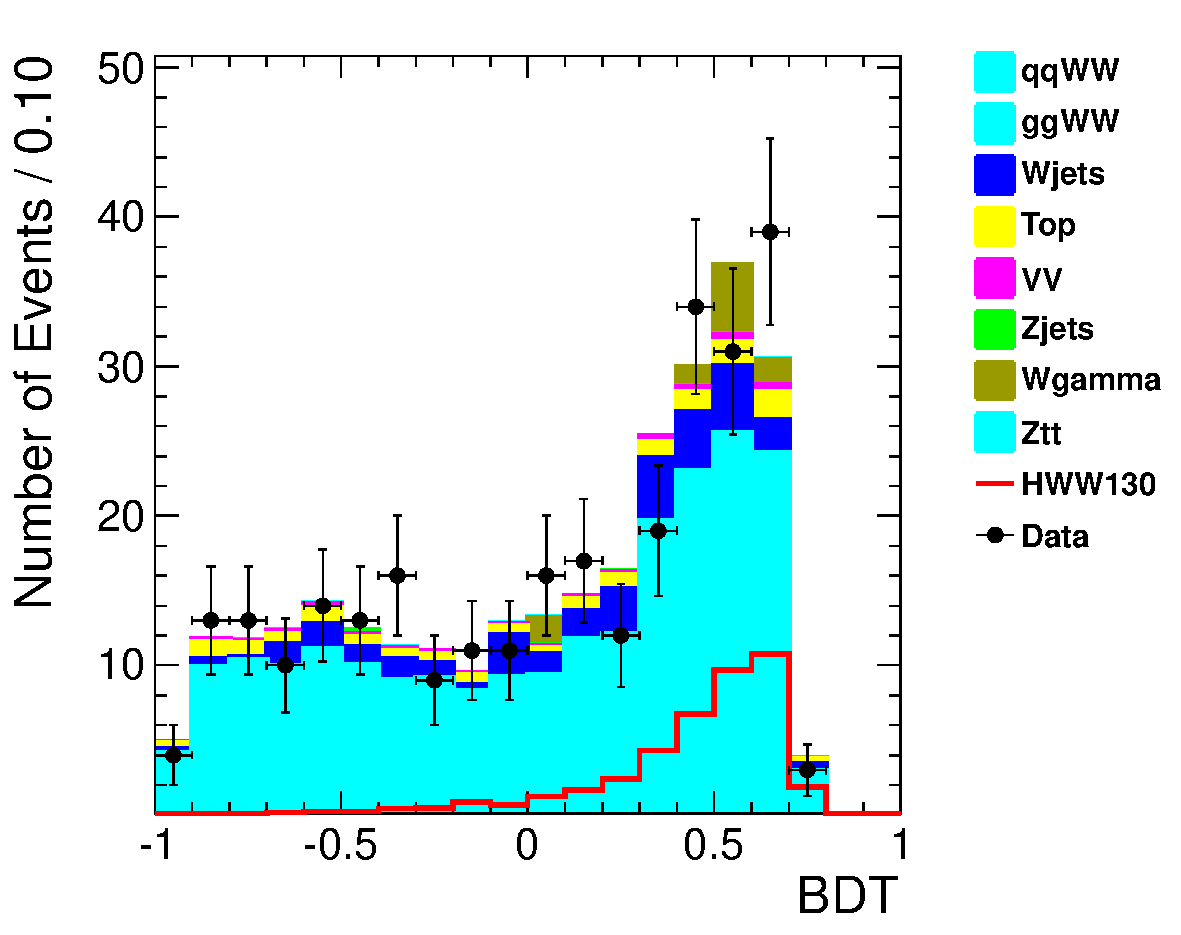
\includegraphics[width=.40\textwidth]{figures/BDT_mH130_0j_of_stack_lin.pdf}}
\subfigure[]{
\centering
\label{subfig:mva_130_0j_sf_4700pb}
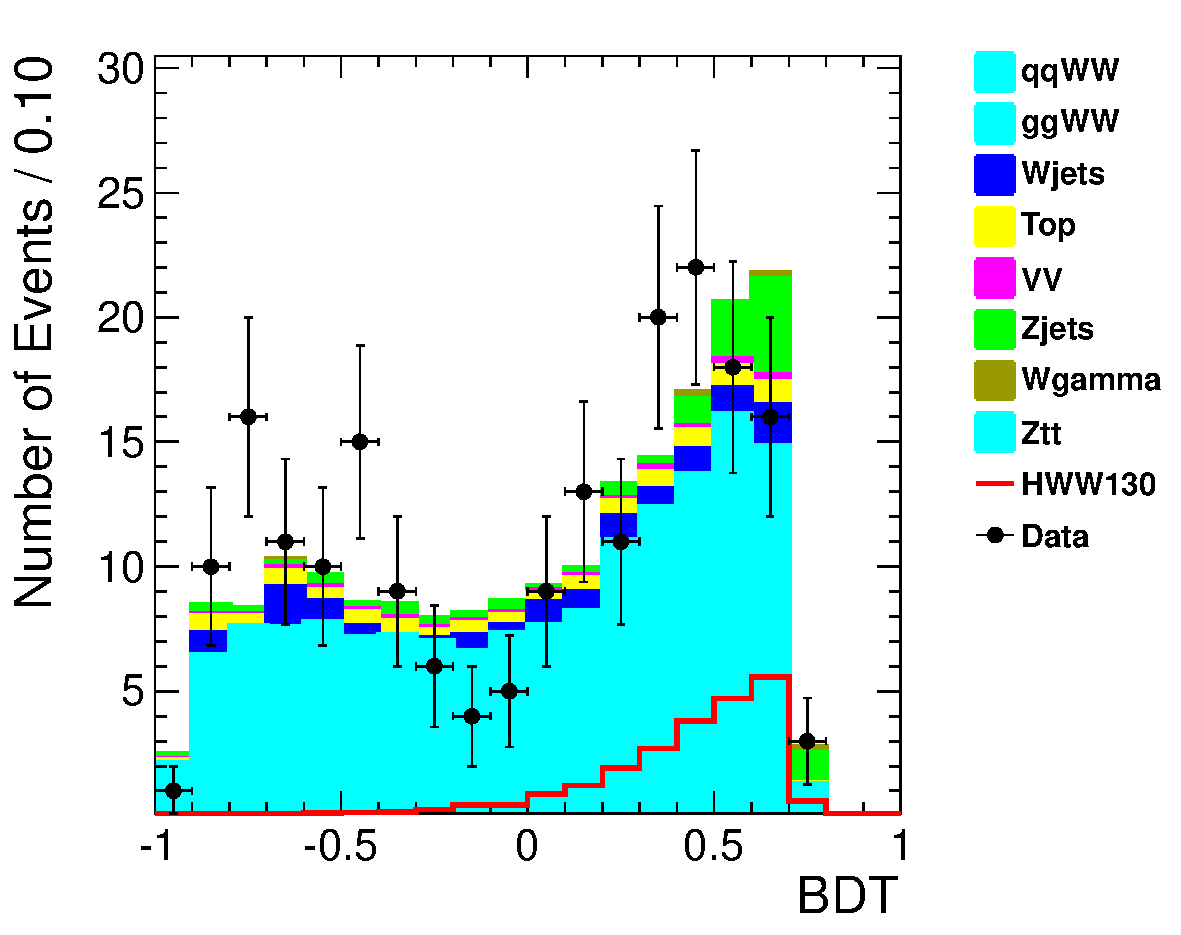
\includegraphics[width=.40\textwidth]{figures/BDT_mH130_0j_sf_stack_lin.pdf}}
\subfigure[]{
\centering
\label{subfig:mva_130_1j_of_4700pb}
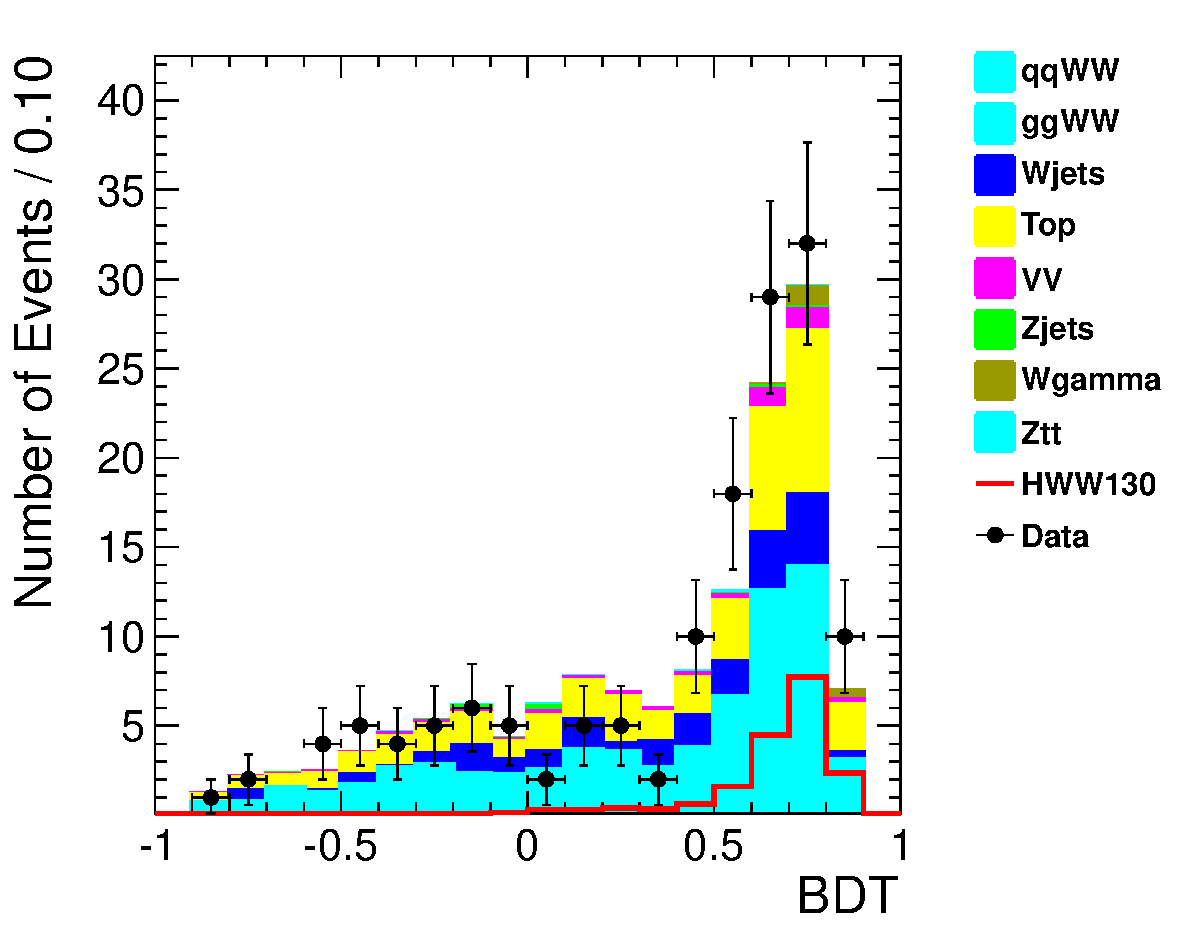
\includegraphics[width=.40\textwidth]{figures/BDT_mH130_1j_of_stack_lin.pdf}}
\subfigure[]{
\centering
\label{subfig:mva_130_1j_sf_4700pb}
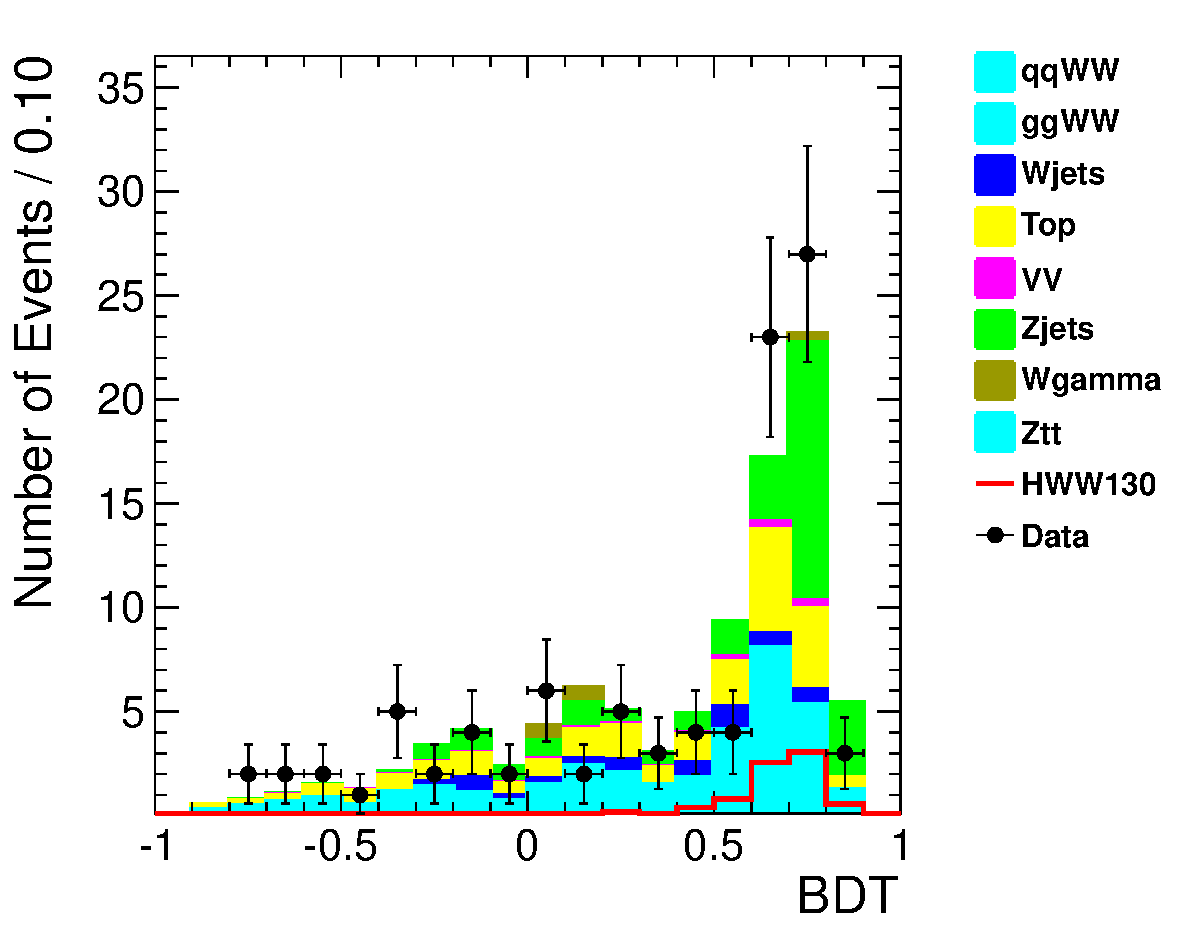
\includegraphics[width=.40\textwidth]{figures/BDT_mH130_1j_sf_stack_lin.pdf}}
\caption{
MVA output for $m_H$=130 GeV corresponding to \intlumi:
0-jet OF \subref{subfig:mva_130_0j_of_4700pb},
0-jet SF \subref{subfig:mva_130_0j_sf_4700pb},
1-jet OF \subref{subfig:mva_130_1j_of_4700pb},
1-jet SF \subref{subfig:mva_130_1j_sf_4700pb}
.}
\label{fig:mva_130_4700pb}
\end{figure}

\begin{figure}[!hbtp]
\centering
\subfigure[]{
\centering
\label{subfig:mva_140_0j_of_4700pb}
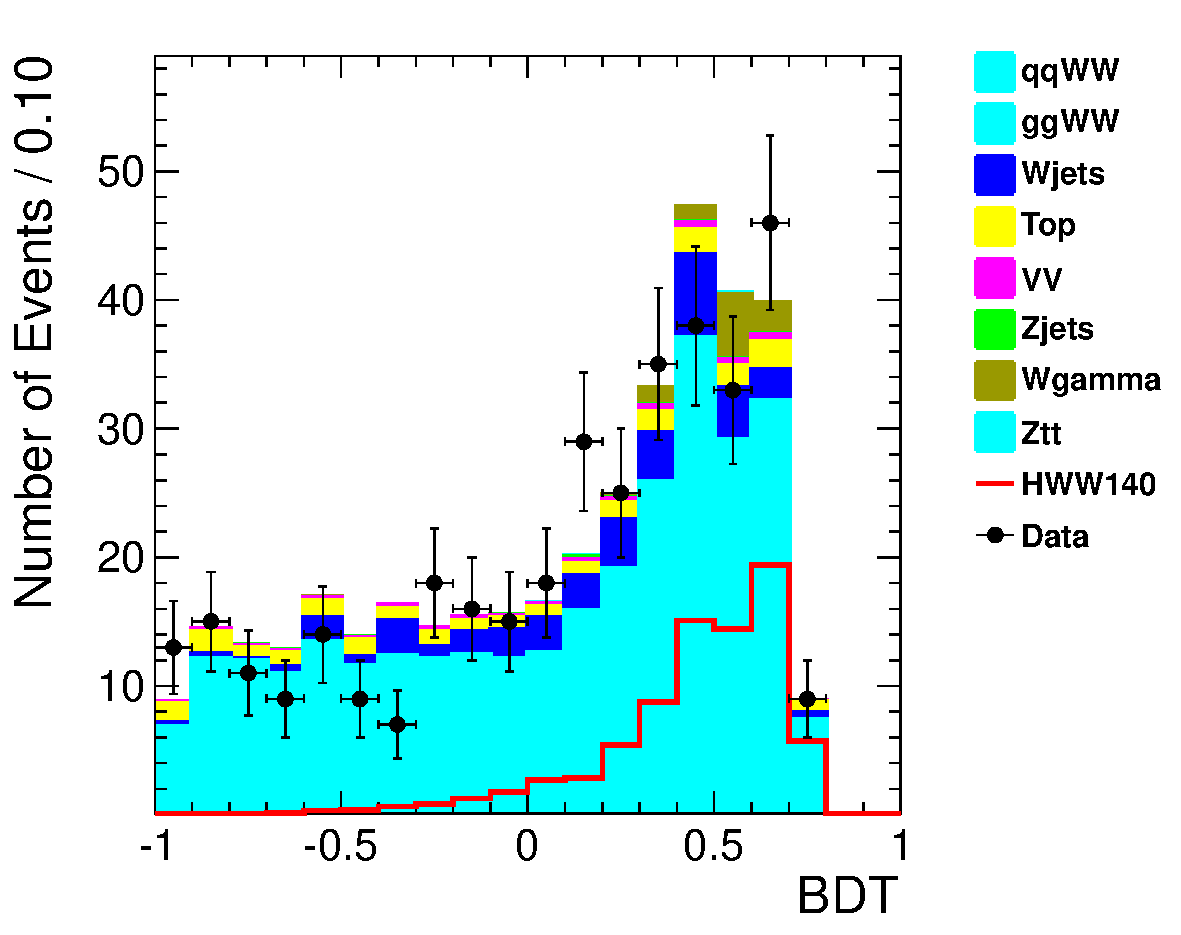
\includegraphics[width=.40\textwidth]{figures/BDT_mH140_0j_of_stack_lin.pdf}}
\subfigure[]{
\centering
\label{subfig:mva_140_0j_sf_4700pb}
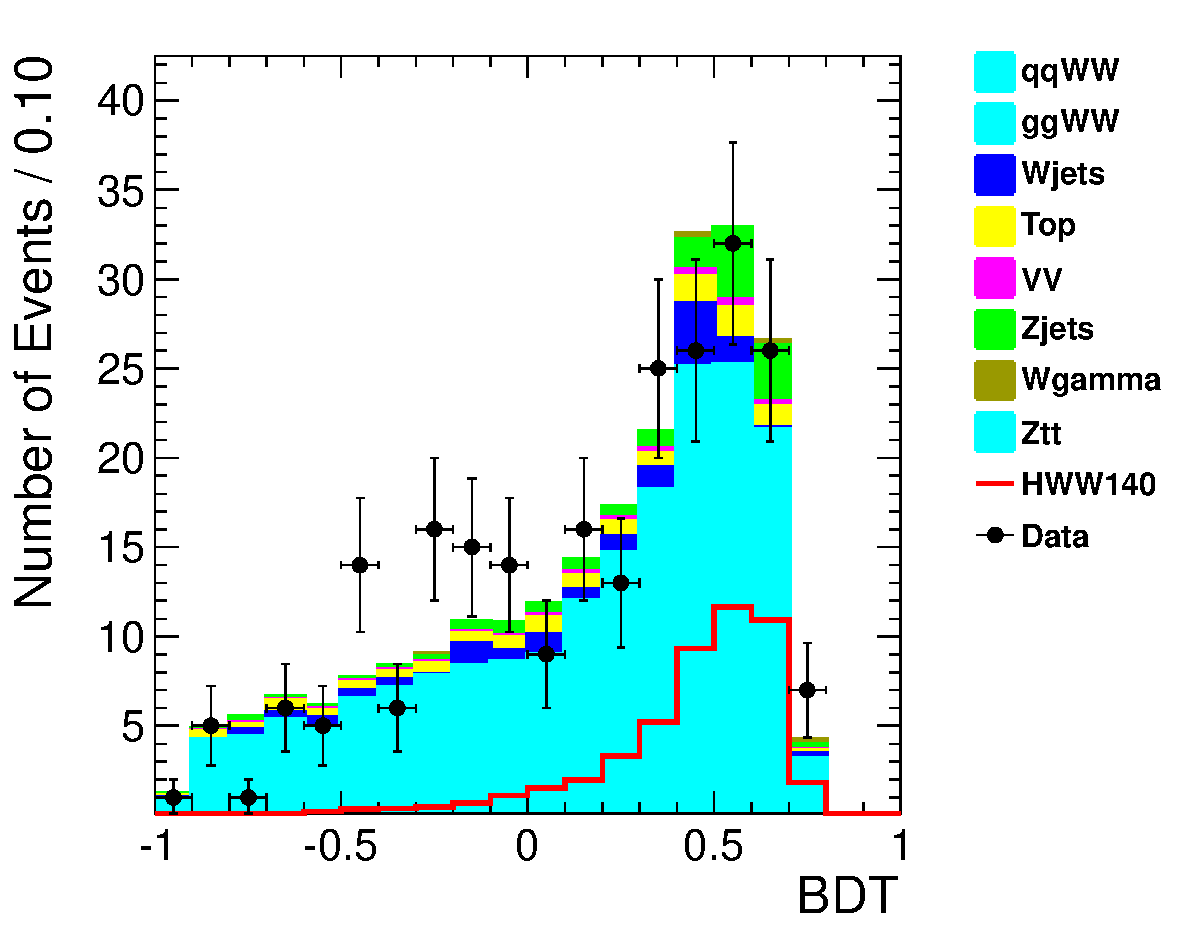
\includegraphics[width=.40\textwidth]{figures/BDT_mH140_0j_sf_stack_lin.pdf}}
\subfigure[]{
\centering
\label{subfig:mva_140_1j_of_4700pb}
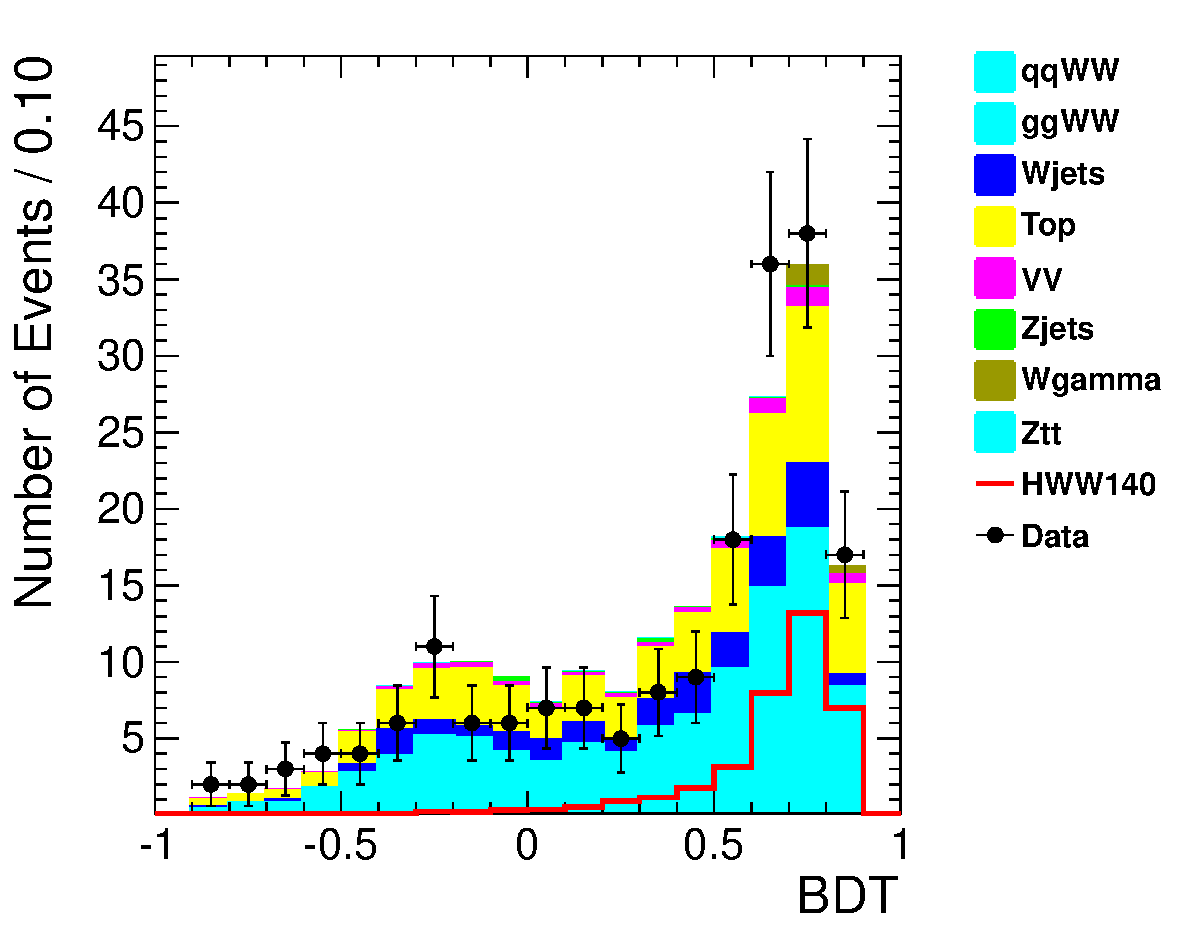
\includegraphics[width=.40\textwidth]{figures/BDT_mH140_1j_of_stack_lin.pdf}}
\subfigure[]{
\centering
\label{subfig:mva_140_1j_sf_4700pb}
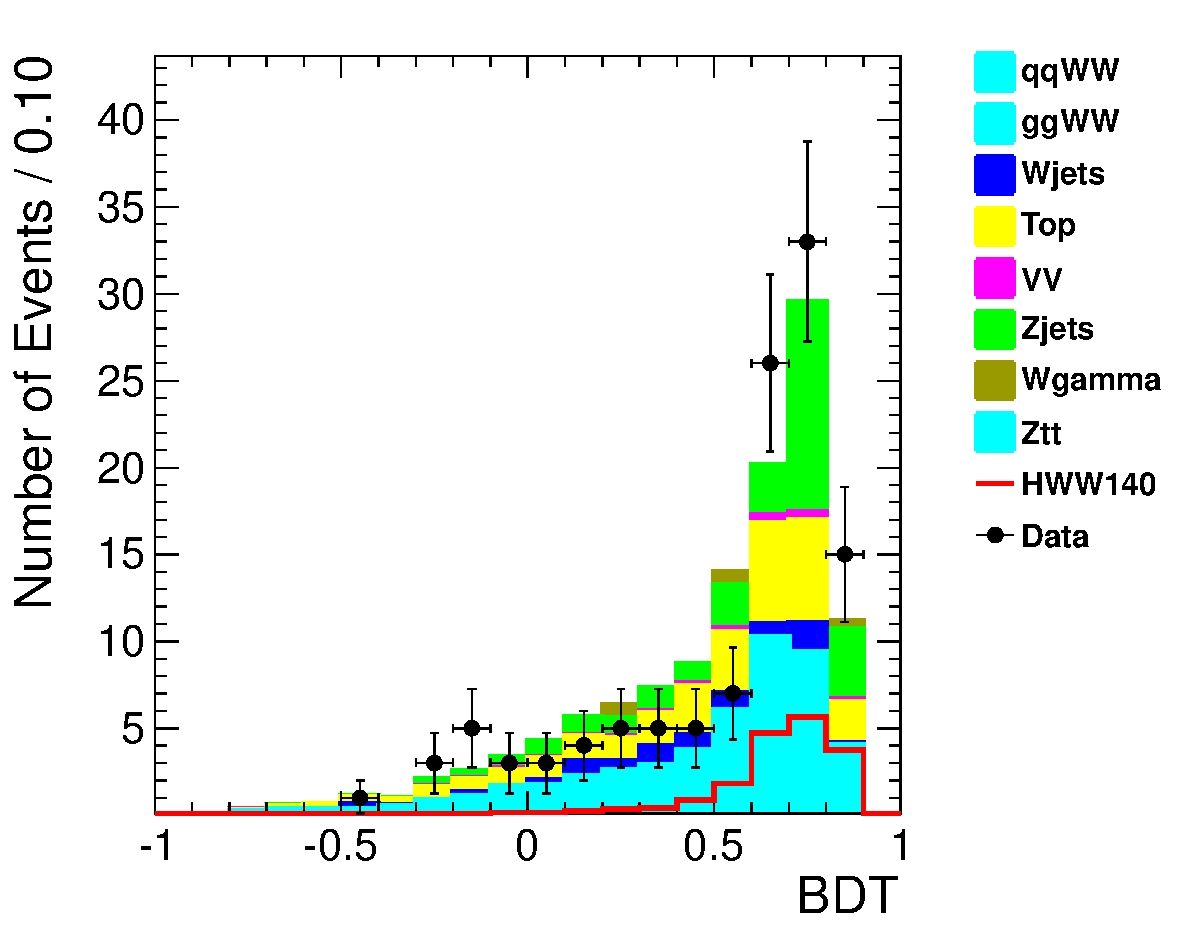
\includegraphics[width=.40\textwidth]{figures/BDT_mH140_1j_sf_stack_lin.pdf}}
\caption{
MVA output for $m_H$=140 GeV corresponding to \intlumi:
0-jet OF \subref{subfig:mva_140_0j_of_4700pb},
0-jet SF \subref{subfig:mva_140_0j_sf_4700pb},
1-jet OF \subref{subfig:mva_140_1j_of_4700pb},
1-jet SF \subref{subfig:mva_140_1j_sf_4700pb}
.}
\label{fig:mva_140_4700pb}
\end{figure}
